\section{LoRa module}
In order to test the LoRa SX1278 module, one wrote a small program to test send and receive functions from LoRa module, with the usage shown in figure \ref{fig:loratest}.

\begin{figure}[H]
	\centering	
	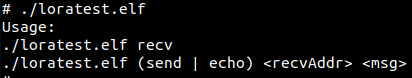
\includegraphics[width=0.6\textwidth]{13tests/lora/loratest}
	\caption{Test LoRa module.}
	\label{fig:loratest}
\end{figure}

Using two LoRa modules, one was connected to a Raspberry Pi in\linebreak
\verb|tomas-abreu|'s computer with local address defined as \verb|0xbb|, the other was connected to another Raspberry Pi in \verb|fernandes|'s computer with local address \verb|0xcc|.

One tested the read and send functions of the module, firstly by waiting for a message, as shown in figure \ref{fig:loratest_recv}.

\begin{figure}[H]
	\centering	
	\includegraphics[width=0.6\textwidth]{13tests/lora/BB_recv_wait}
	\caption{Test LoRa module: waiting for receive.}
	\label{fig:loratest_recv}
\end{figure}

In figure \ref{fig:loratest_send} (a) the device \verb|0xcc| sends the message \verb|"Hello from 0xCC"| to the device \verb|0xbb|, presenting all the attributes, from the source address, \verb|'from'| field, to the destination address, \verb|'to'| field, including also message attributes, as the \verb|msgID|, \verb|msgLength| and the \verb|msg| itself.

In figure \ref{fig:loratest_send} (b) is shown the receiver side, receiving the message correctly, with error 0, and presenting all the attributes from the received message, matching all that were sent by the sender.

\begin{figure}[H]%
	\centering
	\subfloat[\centering Sender side ]{{\includegraphics[width=6.25cm]{13tests/lora/CC_send}}}%
	\qquad
	\subfloat[\centering Receiver side ]{{\includegraphics[width=6.25cm]{13tests/lora/BB_recv}}}%
	\caption{Test LoRa module: send message from 0xcc to 0xbb.}%
	\label{fig:loratest_send}%
\end{figure}
	
As previously seen, the SPI interface works by sending two bytes in a row, depending on what operation it is: read or write. In figure \ref{fig:loratest_sck_nss} is seen the clock signal (SCK, in red) and the slave select signal (NSS, in yellow).

\begin{figure}[H]
	\centering	
	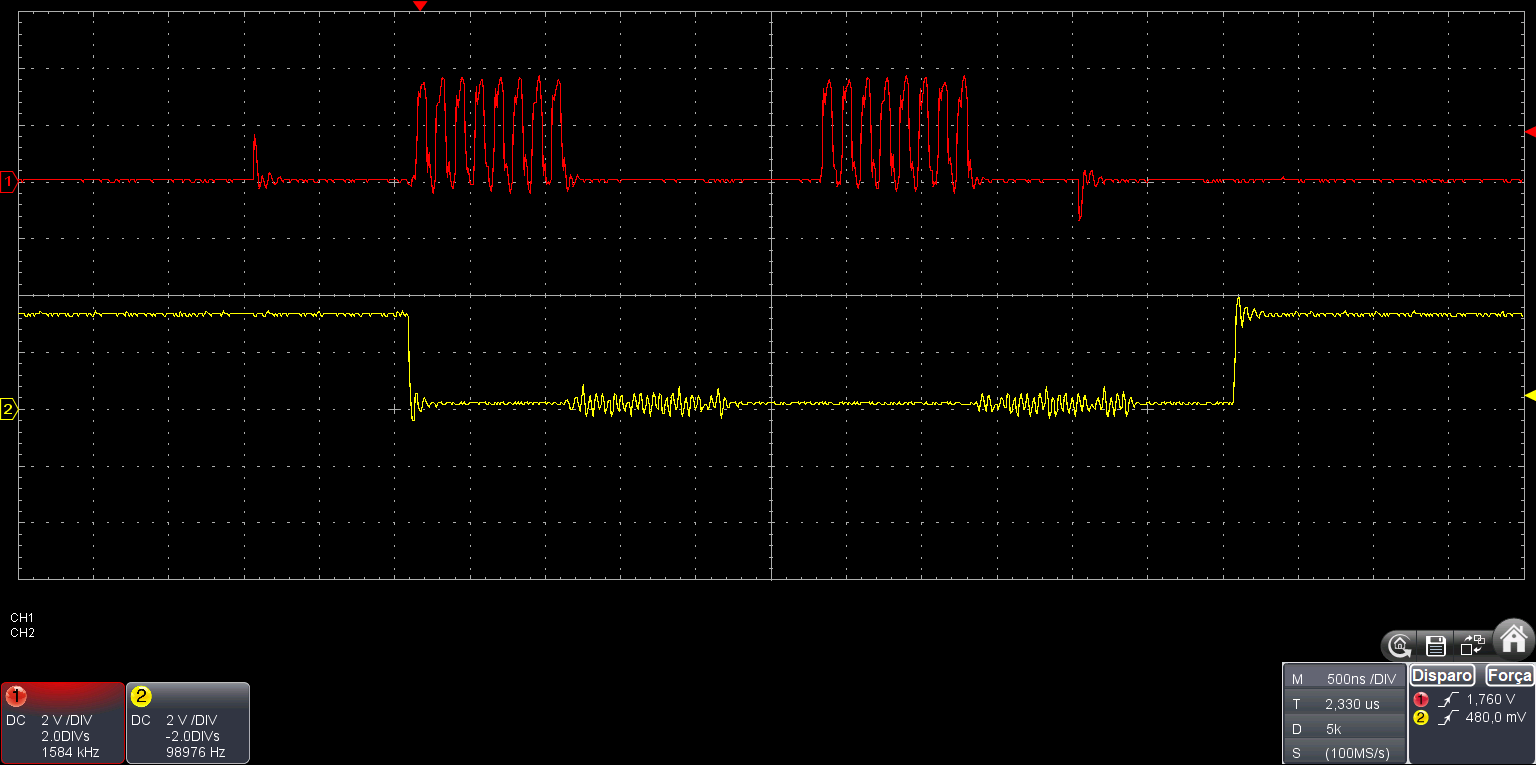
\includegraphics[width=1\textwidth]{13tests/lora/SCK_CS}
	\caption{Test LoRa module: SCK (in red) and NSS (in yellow) signals.}
	\label{fig:loratest_sck_nss}
\end{figure}

When the NSS goes to low, a transfer is started, with the master generating SCK. For each byte are generated 8 pulses of clock, 1 pulse per bit sent. Due to overhead and delays introduced by the software, there is a gap between the two bytes sent, where the NSS signal is still low but the SCK is not being generated. When NSS goes high, the transfer is over.

%**********************************************************
\section{TSL2581}

%**********************************************************
\section{PWM control}
In order to test PWM control, one wrote a small program to test the generation of a PWM signal at 50 Hz with a variable duty cycle, with the usage shown in figure \ref{fig:loratest}. The duty cycle received is a value from 0 to 1.

\begin{figure}[H]
	\centering	
	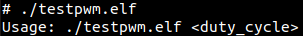
\includegraphics[width=.5\textwidth]{13tests/pwm/testpwm}
	\caption{Test PWM control.}
	\label{fig:testpwm}
\end{figure}

In figure \ref{fig:pwm_50} one defined duty cycle as \verb|0,5| (\verb+50 %+). As seen in the Implementation phase, the \verb+RANGE = 67500+ , so considering the inserted duty cycle, the PWM pulse ratio should be \verb|RANGE*0,5 = 33750|, as shown in figure \ref{fig:pwm_50} (a), in the field \verb|PWM data|.

In figure \ref{fig:pwm_50} (b) is shown the generated PWM signal, with time division of \verb+5 ms+ per division, adding up to \verb+20 ms+ per period, which is referent to a 50 Hz wave.

\begin{figure}[H]%
	\centering
	\subfloat[\centering Set duty cycle to 50\%. ]{{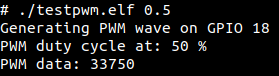
\includegraphics[width=6.25cm]{13tests/pwm/pwm_50}}}%
	\qquad
	\subfloat[\centering Generated PWM signal. ]{{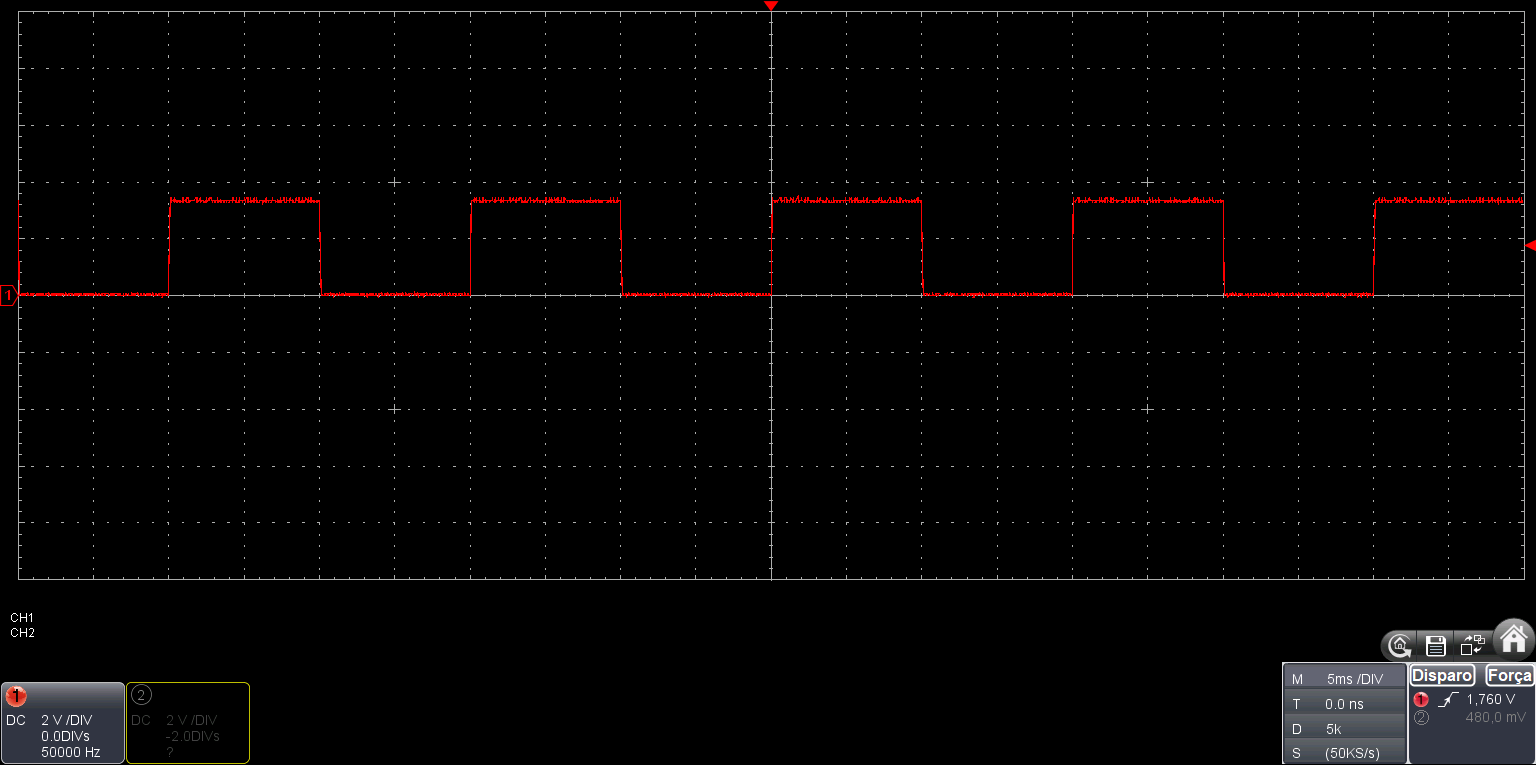
\includegraphics[width=12cm]{13tests/pwm/Duty_50}}}%
	\caption{Test PWM control: PWM at 50\% duty cycle.}%
	\label{fig:pwm_50}%
\end{figure}

In figure \ref{fig:pwm_25} is shown the a PWM generated signal with \verb+25 %+ duty cycle, with output on the GPIO 18. In figure \ref{fig:pwm_25} (a) one can check that the field \verb|PWM data| is equal to \verb+RANGE*0,25+.

\begin{figure}[H]%
	\centering
	\subfloat[\centering Set duty cycle to 25\%. ]{{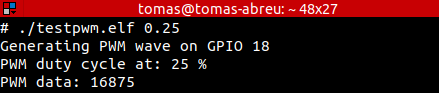
\includegraphics[width=6.25cm]{13tests/pwm/pwm_25}}}%
	\qquad
	\subfloat[\centering Generated PWM signal. ]{{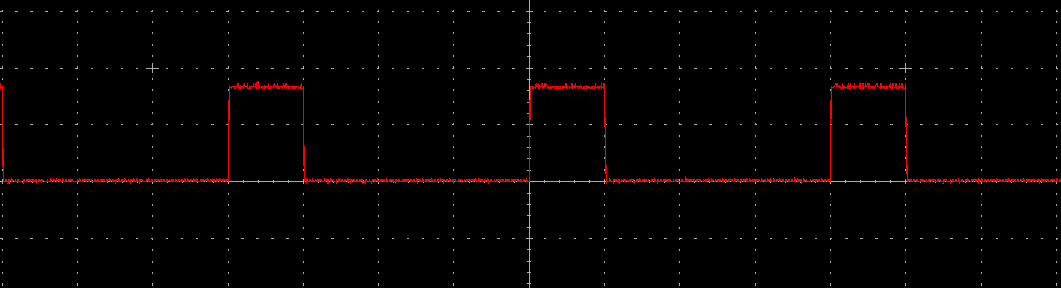
\includegraphics[width=12cm]{13tests/pwm/Duty_25}}}%
	\caption{Test PWM control: PWM at 25\% duty cycle.}%
	\label{fig:pwm_25}%
\end{figure}

%**********************************************************
\section{Motion Detector}